% Chapter 4
\chapter{Network Reconfiguration Software} % Write in your own chapter title
\label{Chapter 4}
\lhead{} % Write in your own chapter title to set the page header

\section{Overview}
This chapter discusses the software developed in this thesis. First, this chapter discusses the procedures involved in network reconfiguration and the features required to achieve that goal. Next, the features are discussed in terms of the software functionality that needs to be implemented. Finally, the chapter discusses how the different functionality is grouped into software modules. The specifics of how each module works is described in Chapter 5.

\section{Approach}
To achieve network reconfiguration functionality within WiSARDNet, the following features are required: 

\begin{itemize}
	\item The user needs an up to date understanding of a WSN's configuration.
	\item The user needs to be able to specify the desired configurations or features they want to make to a set or subset of WSN nodes.
	\item Users need to be able to communicate configuration changes to the WSN. 
	\item The WSN needs to execute the new behaviors that the user specifies.
	\item The system needs protections that ensure continued and correct WSN operation.
\end{itemize} 

As was shown in Chapter 2, there are many ways that other WSN platforms have approached network reconfiguration. For the work in this thesis, a database abstraction is used as the general approach for structuring WSN reconfiguration. The specific abstraction used is that the WSNs in WiSARDNet can be viewed as a database of dynamic heterogeneous behaviors. By viewing the WSNs from a database perspective, queries and inserts become the language that users can use to interact with the WSN. The database paradigm simplifies the complexity of WiSARDNet and guides the design of WSN reconfiguration.

In addition to the database abstraction, another abstraction is used to approach WSN reconfiguration. As described in Chapter 3, the components that comprise a WiSARD are represented in the WiSARDNet PostgreSQL database as individual devices with deployments that describe their current state. Since a WiSARD is a collection of these physical devices, it is useful to represent the device deployments as WiSARD objects. This is especially true given the number of database relationships that are managed, such as those to parent deployments, device types, sites. Figure \ref{fig:wisard_object} shows an example of how a WiSARD encapsulates multiple related deployments. 

% wisard abstraction
\begin{figure}[H]
	\centering
	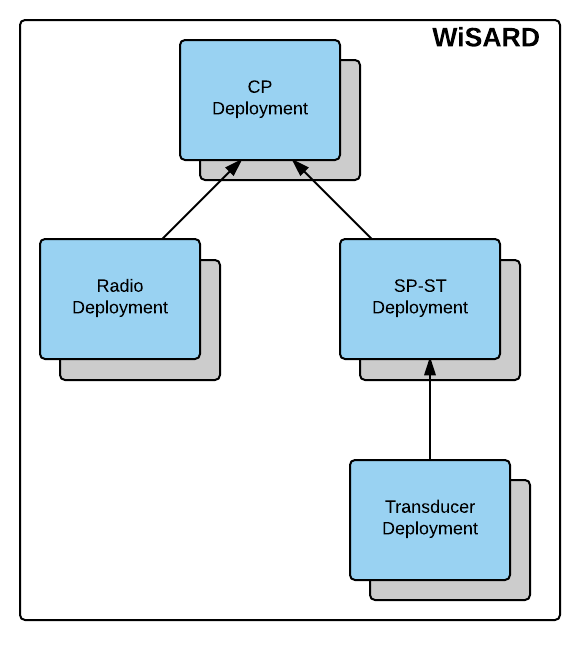
\includegraphics[width=.6\textwidth]{figures/wisard_abstraction_example.png}
	\caption{An example of the WiSARD abstraction used to encapsulate multiple related device deployments. Each arrow represents a deployment record's reference to its parent deployment.}
	\label{fig:wisard_object}
\end{figure}

% wisard database representation
\begin{figure}[H]
	\centering
	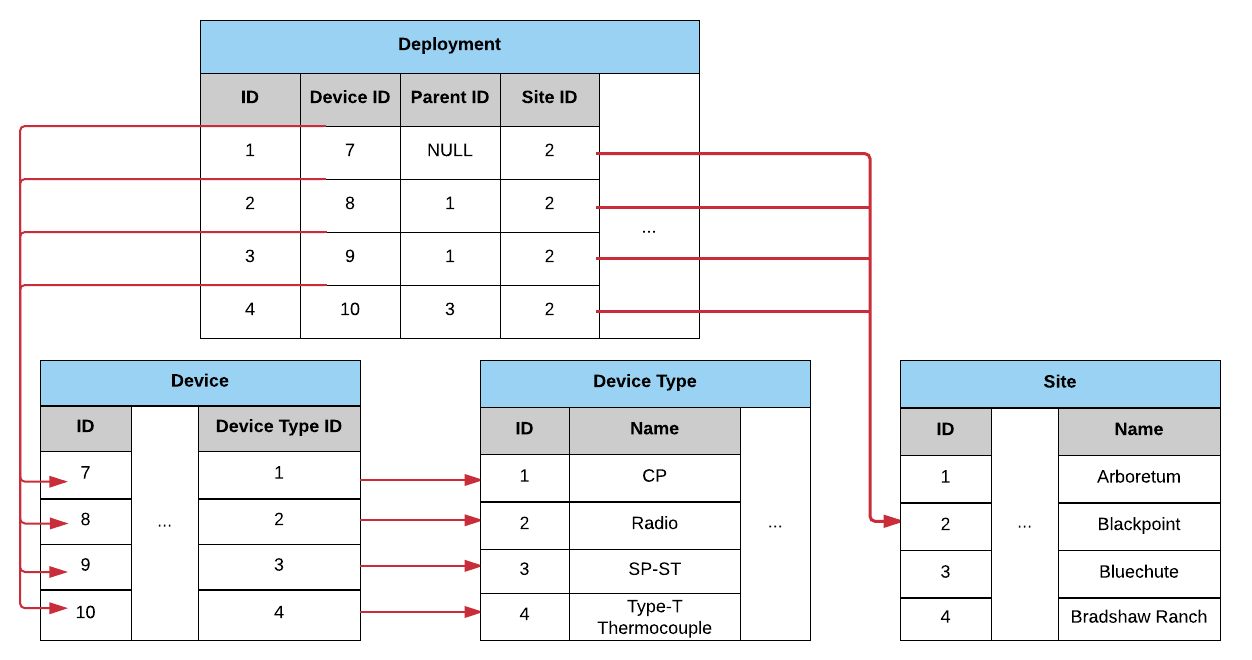
\includegraphics[width=\textwidth]{figures/wisard_abstraction_example_database.png}
	\caption{Database representation of example WiSARD abstraction from Figure \ref{fig:wisard_object}. The arrows illustrate foreign key references between records in different tables.}
	\label{fig:wisard_object_database}
\end{figure}

Using WiSARD objects to encapsulate multiple related device deployments means that a WSN can be reconfigured by updating sets of WiSARDs rather than many individual deployments. The database abstraction of the WSNs and the WiSARD abstraction of the WSN node devices together provide the conceptual foundation for the reconfiguration features to be implemented in software. The WiSARD abstraction is implemented in code as a Java class. Each instance of the WiSARD class encapsulates all of the device deployments of a WiSARD object as shown in Figure \ref{fig:wisard_object}. Instances of the WiSARD class provide methods for accessing records referenced by deployment foreign keys, similar to navigation properties in Object Relational Mapping (ORM) objects. For example, devices in a WSN are deployed at locations where a researcher would like to gather data. A Site database table was created in order to store information related to such deployment locations. One of the ORM-like methods that a WiSARD object provides is one that will return the Site record referenced by the WiSARD deployments. In addition to the WiSARD class, there are classes for encapsulating other tables in the database, including the Site Table. When a WiSARD returns a deployment's Site record, it is in the form of an instance of the Site class. The database tables and their related Java classes are discussed in further detail in the following Section. 

%%%%%  FINISH THIS SECTION  %%%%

\section{Solution Description}
Implementing WSN reconfiguration functionality into an existing software system requires that new code modules be developed that account for all of the known use cases and as many future use cases as possible. A practical example is a scenario where a researcher wants all soil moisture transducers attached to WSN nodes in a specific region to be sampled at twice their current sampling rate. Performing this procedure involves the user specifying the region and sensor types needed to produce a matching set of WSN nodes, and that he/she wants the sampling rate of those transducers to be changed. The software needs to validate that there are no conflicts between that user's requested changes and the existing operational configurations of the node. Finally, the nodes will each be signaled via command packets, execute the specified change in configuration, and will then alert the user of the changes made.

\subsection{Implementing Functionality}
Each of the features described in the previous section needs to be implemented as software functionality to be used in the WiSARDNet system. This section describes the software tasks for each feature. 

\subsubsection{Identification of WSN Nodes}
Transducer samples, sensor types, WiSARD role information, and hardware metadata are all stored in database tables and are necessary to determine which nodes will need to be reconfigured. The first stage in reconfiguring a WSN is the specification of the node or nodes whose configurations will be modified. This operation begins with a user specifying search criteria for a set of WiSARD that they want to reconfigure. Next, static and dynamic WiSARD information is gathered by querying a set of PostgreSQL database tables that have all of the information that describes a WiSARD. Table \ref{tab:db_tables} shows all of the tables that are queried when searching for WiSARDs and describes the information stored in each table. The results of these queries are then stored in instances of Java objects created for each table.

%%% FIX TABLE REFERENCE %%%

%%% ADD TABLE OF DATABASE TABLES %%%
\begin{table}[H]
	\centering
	\renewcommand{\arraystretch}{1.1}
	\begin{tabu}{|X[2.5,c]|X[8,c]|}
	\hline
	\textbf{Database Table} & \textbf{Description}\\
	\hline
	Device & Stores a record for each device in WiSARDNet\\
	\hline
	Deployment & Stores a record for each deployment of a device\\
	\hline
	DeviceType & Stores a record for each possible type of device\\
	\hline
	DeploymentType & Stores a record for each type of deployment \\
	\hline
	Site & Stores geographic information about each garden site\\
	\hline
	Experiment & Stores a record for each WiSARDNet experiment\\
	\hline
	\end{tabu}
	\caption{A list of the database tables that contain information relevant to WiSARDs}
	\label{tab:db_tables}
\end{table}

The next step in this procedure is to filter all of the queried information against the search criteria that a user has specified. Once a list of WiSARDs that match the search criteria is obtained, the user can specify a new configuration to be applied to each WiSARD in that list. The software which obtains search criteria, translates information from  database tables to Java objects, and filters WiSARDs is described in further detail in the Chapter 5.

\subsubsection{Describing the New Configuration}
A WiSARD's task execution is governed by a set of configuration parameters stored within the device's non-volatile memory; this area of memory is called the task control block. Changing a device's behavior is achieved by overwriting specific values within the task control block with values that represent different behaviors. The user must describe the changes to the system so that the correct fields in the task control block can be overwritten with appropriate values corresponding to the new behaviors. This is achieved by encoding different behavior or behavior profiles into control sequences which the WiSARDs are able to decipher. 

\subsubsection{Validating the New Configuration}
As the number of configuration changes and the number of affected WSN nodes increases, the possibility of errors or resource conflicts between experiments also increases. To prevent conflicts, there is a need to validate that the intended changes will not interfere with other experiments each node is associated with. This is achieved with user access control and command validation.

User access control is the process of restricting the access of users to specific pieces of hardware or software based on a set of rules and permissions that govern the extent to which they can interact with the WSN. For example, a researcher should not be allowed to reconfigure another researcher's hardware or reconfigure the WSN in a way that will adversely affect other experiments. User access control in WiSARDNet is achieved by using database tables to store information about users and the WiSARDs they are allowed to change.

Command validation is the process of analyzing the configuration changes a user intends to make to a specified set of WiSARDs and determining whether the change is feasible and safe to make. For example, a user should not be allowed to send a command that will cause a WiSARD to misbehave or prevent it from performing its essential duties. Both user access control and command validation are essential in validating a configuration before execution.

%%% ESSENTIAL DUTIES? %%%

\subsubsection{Command Synthesis}
Once the user has specified a new configuration, command packets are automatically generated. A command packet is a structure which contains a control sequence, configuration parameters, and network routing information which will allow each command to be sent to its intended WiSARD. The control sequences are defined by software classes, the command parameters are obtained from the user's configuration specifications, and the routing information is obtained from the list of WiSARD objects. Once generated, the command packets are added to MQTT messages and flushed from an MQTT publisher client at the RTDC to the MQTT broker at the destination garden server. Each garden server has a WiSARD client which retrieves command packets from the local MQTT broker and sends them into the WSN via the hub node. 

\subsubsection{Executing the Reconfiguration}
When a WiSARD receives a command message from a parent node, the WiSARD parses the command message and schedules a task to execute the command. When a WiSARD executes a command, a report message is created and sent back through the network to the RTDC. The report message will confirm that the task was successfully executed or report that it failed if the task did not execute successfully.

\subsubsection{Verifying the New Configuration}
All data generated by a WSN is sent to the RTDC in the form of data streams. Each transducer reports its samples as specific streams defined by the device relationship structure discussed in Chapter 3. A WiSARD also reports diagnostic and error information as data streams in the same manner. After making a configuration change, a WiSARD reports its new configuration through a designated data stream to the RTDC. 

%%% ADD MORE TO THIS LATER %%%

% software modules - WiSARD Browser, Command Generator, Validation
\subsection{Software Modules}
The software implementation of the functionality described in the previous section is grouped into three distinct modules:

\begin{itemize}
	\item Wisard\_Browser\_Module
	\item Cmd\_Generation\_Module
	\item Validation\_Module
\end{itemize}

Wisard\_Browser\_Module contains the functionality that can identify sets of WiSARDs that match a user's search criteria. Additionally, this module is responsible for providing an up to date view of a WSN. The functionality which allows a user to describe a new WSN configuration and signal those changes to the WSN is grouped into Cmd\_Generation\_Module. The functionality which validates the safety of a new configurations, checks for conflicts, and implements user access control into the system is grouped into Validation\_Module. Figure \ref{fig:wisardnet_ci_additions} illustrates the new modules added to the WiSARDNet CI, as well as the existing software systems with which they communicate.

% wisardnet ci additions
\begin{figure}[H]
	\centering
	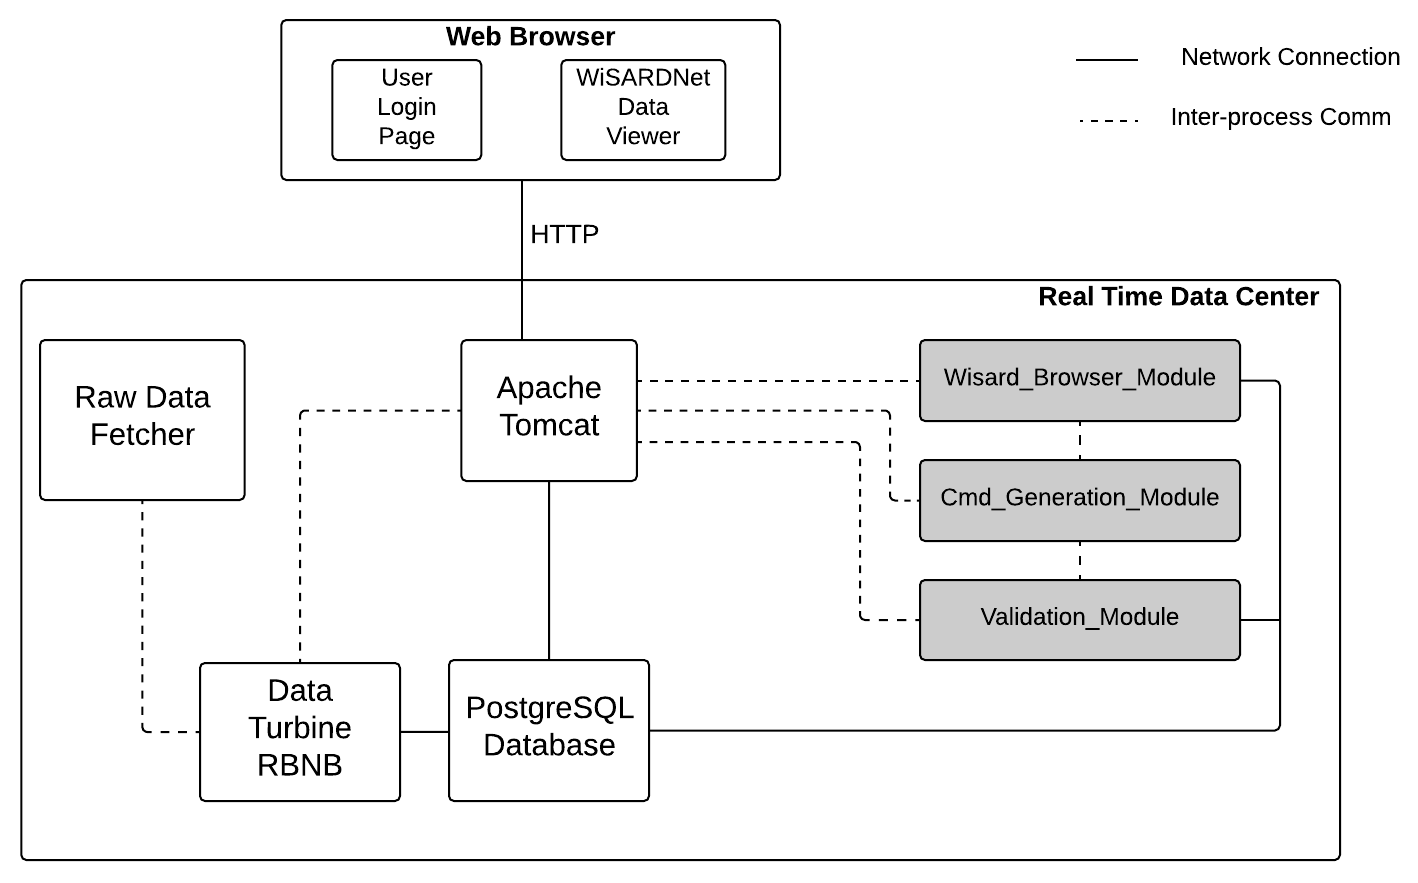
\includegraphics[width=\textwidth]{figures/wisardnet_added_modules.png}
	\caption{The software modules being added to the WiSARDNet cyberinfrastructure for WiSARD reconfiguration are shown in the shaded boxes. }
	\label{fig:wisardnet_ci_additions}
\end{figure}

Each software module contains separate functionality, but they interact and share information with each other as well as the other components of WiSARDNet. Wisard\_Browser\_Module interacts with the web portal user interface, it gathers information about the WSN nodes from the PostgreSQL database, and provides sets of WiSARDs to the other modules. Cmd\_Generation\_Module interacts with the WiSARDNet web portal to generate commands based on a user's input. Additionally, it accesses the list of WiSARDs that Wisard\_Browser\_Module produces. This module accesses the PostgreSQL database to enable stored behaviors to be turned into commands. Lastly, this module provides information to Validation\_Module so that the commands can be verified. Validation\_Module gets session variables from the web portal to authenticate users. It also takes in a set of commands from Cmd\_Generation\_Module, that can validate and report its results.  To verify that the user is permitted to run a specified command, the user and command need to be compared against permission records stored in PostgreSQL database tables. These tables are discussed in detail in Chapter 5.

In summary, the functionality is grouped into three distinct software modules: Wisard\_Browser\_Module, Cmd\_Generation\_Module, and Validation\_Module. These modules need to be able to interact with the different components of the WiSARDNet CI as well as with each other. The software implementations of the modules are discussed in Chapter 5.